
\chapter{Anforderungserhebung}\label{sec:chapter5}
In diesem Kapitel werden die Anforderungen an den in Kapitel 5 folgenden Vergleich der imperativen und deklarativen Modellierung für SE-Prozessmodelle erhoben. Hierfür werden zunächst in Kapitel 4.1 die Vergleichskriterien vorgestellt und erläutert. 

\section{Vergleichskriterien}\label{sec:chapter5:Vergleichskriterien}

Bisher gibt es nur wenige Arbeiten, welche sich mit deklarativen Prozessmodellierungssprachen und insbesondere mit dem Vergleich von imperativen und deklarativen Prozessmodellierungssprachen beschäftigen. Aus diesem Grund soll in der vorliegenden Arbeit ein Vergleich der Anwendbarkeit zwischen deklarativen und imperativen Prozessmodellierungssprachen im Kontext von Softwareentwicklungsprozessen durchgeführt werden. Hierbei soll die Eignung der beiden Prozessmodellierungssprachen für die Modellierung beurteilt werden. Weiterhin sollen die Stärken und Grenzen der beiden Modellierungssprachen aufgezeigt werden und es soll dadurch herausgefunden werden, ob eine der beiden Modellierungssprachen über eine bessere Anwendbarkeit bei der Modellierung verfügt als die andere \cite{list2006evaluation}.\newline
Hierfür sollen die imperativen und deklarativen Prozessmodelle, welche für die drei Softwareentwicklungsprozesse Scrum, Open UP und V-Modell-XT erstellt werden im Hinblick auf verschiedene Vergleichskriterien untersucht werden. Da es sich bei Scrum um ein leichtgewichtiges Softwareentwicklungsprozessmodell, beim V-Modell XT um ein schwergewichtiges Softwareentwicklungsprozessmodell und bei Open UP um ein Softwareentwicklungsprozessmodell handelt, welches sich in der Mitte zwischen leichtgewichtig und schwergewichtig befindet, eignen sich diese drei besonders gut, zum Vergleichen der imperativen und deklarativen Modellierung für unterschiedlich große Metamodelle. Außerdem liegen den in imperativer und deklarativer Modellierungssprache zu erstellenden Prozessmodellen so jeweils die gleichen Metamodelle zugrunde, was eine objektive Bewertung für den Vergleich gewährleistet \cite{list2006evaluation}. \newline

Es sollen die imperativen und deklarativen Modellierungssprachen im Hinblick auf deren Erfüllung der in Kapitel 3.1.1 vorgestellten \textit{Grundsätze ordnungsgemäßer Modellierung} untersucht werden, da durch deren Einhaltung die Qualität, Klarheit und Konsistenz der Prozessmodelle gesichert wird \cite{freund2007}. Somit lässt sich hierdurch die Eignung der beiden Prozessmodellierungssprachen sehr gut überprüfen. Denn falls eine von beiden Prozessmodellierungssprachen die Modellierungsgrundsätze wesentlich schlechter einhalten kann, als die andere, so ist sie zum Modellieren deutlich weniger geeignet, da die hierdurch entstandenen Prozessmodelle geringere Qualität, Klarheit und Konsistenz aufweisen. Hierfür werden nachfolgend die erstellten Prozessmodelle im Hinblick auf \textit{Richtigkeit}, \textit{systematischen Aufbau}, \textit{Relevanz}, \textit{Klarheit}, \textit{Wirtschaftlichkeit} und \textit{Vergleichbarkeit} verglichen. Hierfür werden nachfolgend für jeden Modellierungsgrundsatz verschiedene Kriterien festgelegt, mit deren Hilfe die Einhaltung der Modellierungsgrundsätze für die jeweilige Modellierungssprache in Kapitel 5 überprüft wird. \newline

\subsection{Richtigkeit}
Die Richtigkeit der Prozessmodelle soll verglichen werden. Hierbei soll die syntaktische und semantische Richtigkeit der Prozessmodelle untersucht werden. Die syntaktische Korrektheit soll dahingehend untersucht werden, ob sich die jeweiligen Modelle unter Einhaltung der Modellierungsregeln der jeweiligen Prozessmodellierungssprache erstellen lassen. Bei der semantischen Korrektheit der Prozessmodelle soll verglichen werden, in wie weit die mit deklarativer bzw. imperativer Prozessmodellierungssprache erstellten Prozessmodelle dem zugrunde liegenden Metamodell gegenüber vollständig und konsistent sind. Denn falls wesentliche Aspekte des Metamodells nicht darstellbar sind, leidet der Nutzen des Prozessmodells erheblich.  \newline


\subsubsection{A 1.1}

Die Überprüfung der syntaktischen Richtigkeit der Modelle soll mit Hilfe der Modellierungstools Signavio und Declare durchgeführt werden. Beide Programme verfügen über eine automatische Überprüfung der syntaktischen Korrektheit der dort erstellten Modelle. Somit soll nach dem Modellieren der jeweiligen Prozessmodelle in den entsprechenden Modellierungstools eine automatische Überprüfung der syntaktischen Korrektheit durchgeführt werden. \newline

\subsubsection{A 1.2}

Zum Vergleich der semantischen Korrektheit soll überprüft werden, ob eine der beiden Prozessmodellierungssprachen die Struktur des Metamodells und das dort beschriebe Verhalten besser abbildet als die andere. Insbesondere soll hier untersucht werden, ob es Grenzen in der Darstellbarkeit der abzubildenden Aspekte des Metamodells gibt \cite{journals95, becker2012prozessmanagement}. \newline


\subsection{Systematischer Aufbau}

Da nicht alle Informationen, wie z.B. Daten und Funktionen in einem Prozessmodell abgebildet werden können, ist die Integration anderer Sichten in das Prozessmodell sehr wichtig, um wirklich alle Informationen aus dem Metamodell abbilden zu können. Hier können Rückschlüsse auf die Eignung zur Modellierung gezogen werden und eventuelle Grenzen der Prozessmodellierungssprache aufgezeigt werden \cite{journals95, freund2007, becker2012prozessmanagement,koch2011}.


\subsubsection{A 2.1}
Um den systematischen Aufbau der imperativen und deklarativen Prozessmodelle zu vergleichen, sollen die Prozessmodelle dahingehend untersucht werden, in wie weit sie die Integration anderer Sichten (d.h. die Darstellung von Artefakten im Prozessmodell) in das Prozessmodell unterstützen und sie Verweise auf bestehende Datenmodelle zulassen. 

\subsection{Relevanz}

Beim Vergleich der Relevanz der Prozessmodelle sollen die mit BPMN bzw. ConDec modellierten Prozessmodelle dahingehend verglichen werden in wie weit es möglich ist die Prozessmodelle mit den minimal relevanten Informationen zu erstellen. Hier kann wiederum die Eignung der beiden Prozessmodellierungssprachen sehr gut verglichen werden, da falls mit einer Prozessmodellierungssprache nicht alle minimal relevanten Informationen des Metamodells abgebildet werden können, ist diese weniger zum Modellieren geeignet \cite{journals95, freund2007,reinshagen2009}. 

\subsubsection{A 3.1}

Hier soll somit ein direkter Vergleich zwischen den imperativen und deklarativen Prozessmodellen durchgeführt werden. Anhand von diesem soll festgestellt werden, ob in einer von beiden Prozessmodellierungssprachen mehr der minimal relevanten Informationen zum Metamodell abgebildet werden können als in der anderen.\newline

\subsection{Klarheit}


Die Prozessmodelle, welche jeweils in imperativer und deklarativer Prozessmodellierungssprache erstellt werden, sollen im Hinblick auf ihre Klarheit untersucht werden. Hierbei soll festgestellt werden, ob es wesentliche Unterschiede bei der Verständlichkeit der Prozessmodelle gibt, wenn diese in imperativer, bzw. deklarativer Prozessmodellierungssprache erstellt wurden. Denn fehlende Verständlichkeit eines Prozessmodells führt dazu, dass das Prozessmodell wenig Nutzen bringt \cite{journals95, freund2007,reinshagen2009}. \newline
In der Studie \cite{gruhn2006adopting} wurden Metriken über den geistigen Aufwand entwickelt, welcher für das Verständnis von BPMN-Notationselementen notwendig ist. Den einzelnen Notationselementen werden dort verschiedene geistige Gewichtungen zugewiesen. Ein Sequenzfluss hat auf Grund des geringen geistigen Aufwandes beim Verstehen eine geistige Gewichtung von 1. Das Exklusive Gateway hat eine geistige Gewichtung von 2, falls es nur zwei ausgehende Kanten hat. Bei drei oder mehr ausgehenden Kanten hat es eine geistige Gewichtung von 3. Das Parallele Gateway hat eine geistige Gewichtung von 4. Einem Inklusiven Gateway wird sogar eine geistige Gewichtung von 7 zugeschrieben \cite{gruhn2006adopting}.\newline
Leider existieren derzeit noch keine Metriken über den geistigen Aufwand beim Verstehen der einzelnen Constraints bei ConDec. Jedoch gibt es bereits Studien (\cite{thesis_maja,haisjackl2014understanding}), welche sich anderweitig mit dem Verstehen von deklarativen Prozessmodellen auseinandergesetzt haben. In Bezug auf diese Studien werden die nachfolgenden Unterkriterien zum Vergleich der \textit{Klarheit} der einzelnen Prozessmodelle erhoben.


\subsubsection{A 4.1}
Es soll die Anzahl an Gateways in BPMN und die Anzahl Constraints in ConDec betrachtet werden. Da alle Gateways in BPMN und alle Constraints in ConDec eine unterschiedliche Sematik haben und diese jeweils verstanden werden muss, kann sich eine hohe Anzahl an Gateways, bzw. Constraints negtiv auf die Verständlichkeit auswirken \cite{gruhn2006adopting, thesis_maja}. \newline
Da die Existenz-Constraints relativ einfach zu verstehen sind \cite{thesis_maja}, sollen sie beim Vergleich in Kapitel 5 mit den Sequenzflusselementen gleichgesetzt werden und haben somit auch in etwa eine geistige Gewichtung von 1 \cite{thesis_maja,haisjackl2014understanding, gruhn2006adopting}. \newline
Da die Constraints in ConDec genau wie die Gateways in BPMN Patterns darstellen, müssten sie ebenfalls alle Werte für die geistige Gewichtung zwischen 2 und 7 annehmen. Da die Constraints jedoch nicht direkt den Gateways in BPMN zugeordnet werden können und sich somit die geistigen Gewichtungen der Gateways nicht auf die Constraints übertragen lassen soll im Vergleich in Kapitel 5 nur die jeweilige Anzahl an Gateways in BPMN mit der Anzahl an Constraints im ConDec-Modell verglichen werden. Es soll somit auch bei den Gateways in BPMN keine Unterscheidung zwischen den Gateways stattfinden \cite{thesis_maja,haisjackl2014understanding, gruhn2006adopting}. \newline
Zudem soll auch die Anzahl an unterschiedlichen Gateways in BPMN und Constraints in ConDec betrachtet werden. Denn sowohl bei BPMN, als auch bei ConDec wurde in Studien herausgefunden, dass gerade die Kombination von vielen verschiedenen Gateways/Constraints einen sehr großen negativen Einfluss auf das Verstehen hat \cite{gruhn2006adopting, thesis_maja,haisjackl2014understanding}. \newline
Somit sollen beim Vergleich in Kapitel 5 die Anzahl an Sequenzfluss/Existenz Constraints, Gateways/Constraints und unterschiedliche Gateways/Constraints bei den deklarativen und imperativen Modellen direkt gegenüber gestellt werden. Hierbei soll das Kriterium höhere Anzahl an Sequenzfluss/Existenz Constraints einfach gewichtet und die Kriterien höhere Anzahl an Gateways/Constraints und unterschiedliche Gateways/Constraints jeweils doppelt gewichtet werden. Das Modell welches sodann die höhere Anzahl aufweist soll als das komplexere Modell eingestuft werden und erfüllt die \textit{Klarheit} dadurch weniger.



\subsubsection{A 4.2}
Zudem soll untersucht werden, ob bei dem mit ConDec erstellten Modell ein klarer Einstiegspunkt mit Hilfe des Init-Constraints dargestellt werden kann. Das Init-Constraint kann bei ConDec nur einer einzigen Aktivität im Modell zugewiesen werden. Kommen mehrere Aktivitäten als Einstiegspunkt im Modell in Frage, so lassen sich diese in ConDec nicht klar kennzeichnen. Es existieren Studien darüber \cite{haisjackl2014understanding}, dass sich dies negativ auf das Verständnis von ConDec Modellen auswirkt. \newline

\subsubsection{A 4.3}
Weiterhin soll hier untersucht werden, ob es wesentliche Unterschiede in der Verständlichkeit der imperativen und deklarativen Prozessmodelle gibt, in Abhängigkeit der Größe des Prozessmodells. Falls es Unterschiede in der Verständlichkeit der Prozessmodelle in Abhängigkeit der Größe des Prozessmodelles gibt, lassen sich hierbei Rückschlüsse auf die Eignung der Prozessmodellierungssprache in Bezug auf große/kleine Modelle ziehen.


\subsection{Wirtschaftlichkeit der Prozessmodelle}

Hier soll untersucht werden, ob sich der Aufwand für die Modellierung bei den beiden Modellierungssprachen erheblich voneinander unterscheidet, da wenn die Erstellung eines Prozessmodells mit einem zu hohen Aufwand verbunden ist, obwohl der spätere Nutzen des Prozessmodells erheblich geringer ist, ist die Modellierung nicht sinnvoll. Dies soll ähnlich wie bei \textit{Klarheit} in Bezug auf die Komplexität des zu erstellenden Modelles und den damit verbundenen geistigen Aufwand für den Modellierer untersucht werden \cite{freund2007, journals95, leimeister2012,mendling2010seven}.\newline


\subsubsection{A 5.1}
Es soll die Anzahl von Gateways in BPMN mit der Anzahl von Constraints in ConDec miteinander verglichen werden und auch die Anzahl unterschiedlicher Gateways/Constraints. Da bei der Verwendung von Gateways/Constraints auf Grund der steigenden Komplexität des Prozessmodelles für den Modellierer ein höherer geistiger Aufwand notwendig ist und somit auch ein größerer Aufwand für das Modellieren, kann sich dies negativ auf die \textit{Wirtschaftlichkeit} auswirken. Weiterhin sind komplexere Modelle auch fehleranfälliger, d.h. wenn der Modellierer einen höheren geistigen Aufwand beim Modellieren leisten muss ist es auch wahrscheinlicher, dass ihm Fehler beim Modellieren passieren \cite{freund2007, journals95, leimeister2012,mendling2010seven}.
Hier sollen die gleichen Kriterien wie bei \textit{A 4.1} beschrieben herangezogen werden.


\subsubsection{A 5.2}
Weiterhin soll hier untersucht werden, ob es wesentliche Unterschiede in der \textit{Wirtschaftlichkeit} der imperativen und deklarativen Prozessmodelle gibt, in Abhängigkeit der Größe des Prozessmodelles. 


\subsection{Vergleichbarkeit}
Bei der Vergleichbarkeit der Prozessmodelle soll untersucht werden, ob die in imperativer, bzw. deklarativer Prozessmodellierungssprache erstellten Prozessmodelle, welchen die gleichen Metamodelle zugrunde liegen, trotzdem vergleichbare Prozessmodelle darstellen \cite{freund2007, journals95, leimeister2012}. Hierfür werden die nachfolgenden Unterkriterien definiert.

\subsubsection{A 6.1}
Die Vergleichbarkeit soll in Bezug auf das Ausführungsverhalten der imperativen und deklarativen Prozessmodelle durch Ausführung der Modelle in den Modellierungstools Siganvio und Declare nach der Modellierung überprüft werden. Hier sollen die Pfade, welche im jeweiligen Modell durchlaufen werden können miteinander verglichen werden und somit soll sichergestellt werden, dass das Verhalten der Modelle gleich ist, wenn bei beiden Modellen die gleichen Pfade durchlaufen werden können \cite{haisjackl2014understanding}.

\subsubsection{A 6.2}
Außerdem soll hier die Größe der jeweiligen Prozessmodelle als Vergleichskriterium herangezogen werden. Hier soll die Gesamtanzahl der notwendigen Elemente zur Darstellung des Prozessmodells verglichen werden. Es soll festgestellt werden, ob bei Verwendung einer imperativen oder deklarativen Prozessmodellierungssprache wesentlich mehr Elemente zur Darstellung des gleichen Prozesses notwendig sind \cite{leimeister2012, journals95, freund2007,reinshagen2009}.

 \subsubsection{A 6.3}
Es soll insbesondere untersucht werden, ob die Abstraktionsgrade der Prozessmodelle sich wesentlich voneinander unterscheiden, d.h. es soll untersucht werden, ob es bei einer der beiden Prozessmodellierungssprachen Grenzen in der Darstellbarkeit gibt.


Eine Übersicht über die Modellierungsgrundsätze und die jeweiligen Vergleichskriterien und Unterkriterien mit ihren Abkürzungen bietet Abbildung \ref{fig:TabelleKriterien}.

\begin{figure}[!htbp]
\begin{center}
  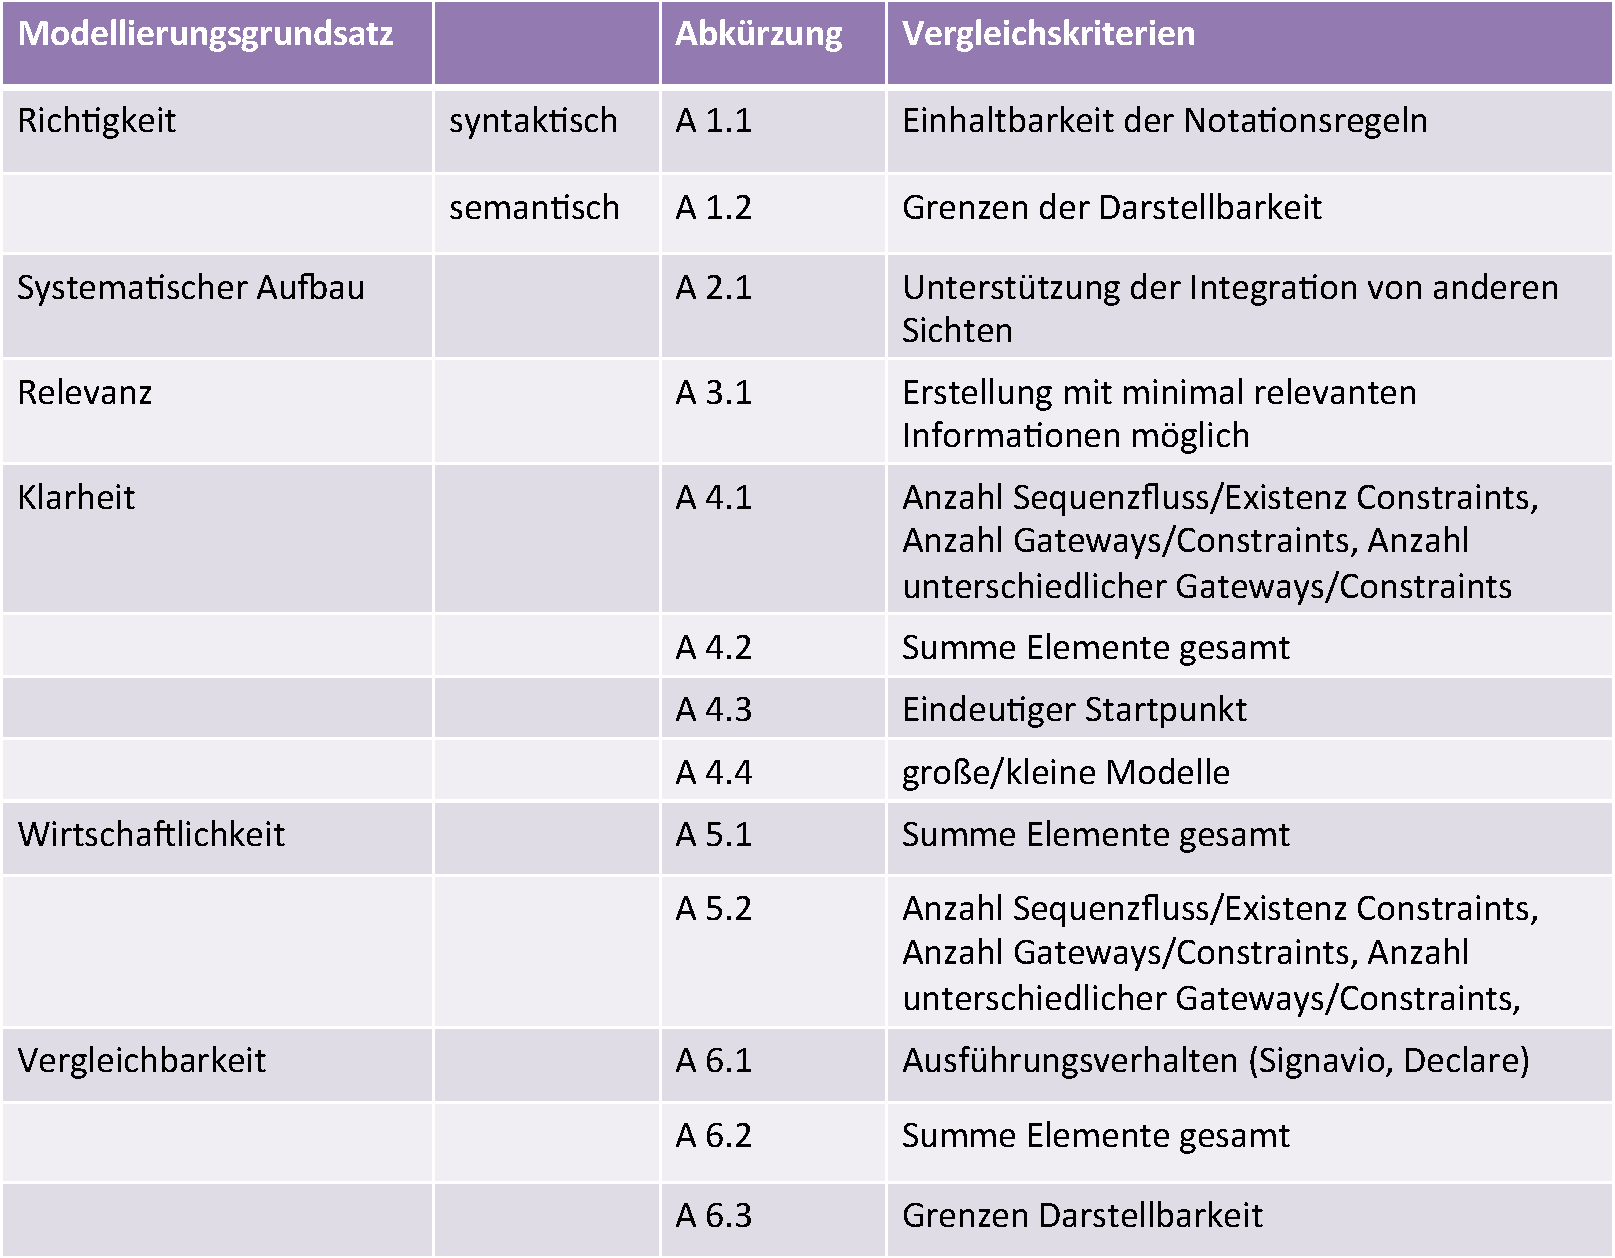
\includegraphics[width=\textwidth]{TabelleKriterien} %pdf, jpg, png...
  \caption{Übersicht Vergleichskriterien}
  \label{fig:TabelleKriterien}
\end{center}
\end{figure}









